\documentclass[11pt]{article}

\usepackage{
    amssymb,
    amsmath,
    amsfonts,
    calc,
    eurosym,
    geometry,
    ulem,
    graphicx,
    caption,
    color,
    setspace,
    sectsty,
    comment,
    footmisc,
    caption,
    % natbib,
    pdflscape,
    subcaption,
    subfiles,
    titling,
    array,
    hyperref,
    booktabs,
    longtable,
    float,
    authblk,
    makecell,
    threeparttable,
    pgfplots}

\usepackage[page]{appendix} % print appendices title

\usepackage[
    backend=biber,
    style=nature,
    date=year,
    doi=true,
    isbn=false,
    url=false,
    eprint=false
]{biblatex}



\AtEveryBibitem{%
  \clearfield{note}%
}
\AtEveryCitekey{\clearlist{publisher}}
\AtEveryBibitem{\clearlist{publisher}}

\usepackage{pgf,tikz}
\usetikzlibrary{arrows, automata}
\usetikzlibrary{shapes.geometric}
\usetikzlibrary{positioning,calc, decorations.pathreplacing}

\usepackage{siunitx}
\newcolumntype{d}{S[input-symbols = ()]}

\normalem

\renewcommand\Affilfont{\small\itshape}

\onehalfspacing
\newtheorem{theorem}{Theorem}
\newtheorem{corollary}[theorem]{Corollary}
\newtheorem{proposition}{Proposition}
\newenvironment{proof}[1][Proof]{\noindent\textbf{#1.} }{\ \rule{0.5em}{0.5em}}

\newtheorem{hyp}{Hypothesis}
\newtheorem{subhyp}{Hypothesis}[hyp]
\renewcommand{\thesubhyp}{\thehyp\alph{subhyp}}

\newcommand{\red}[1]{{\color{red} #1}}
\newcommand{\blue}[1]{{\color{blue} #1}}

\newcolumntype{L}[1]{>{\raggedright\arraybackslash}m{#1}}
\newcolumntype{C}[1]{>{\centering\arraybackslash}m{#1}}
\newcolumntype{R}[1]{>{\raggedleft\arraybackslash}m{#1}}
\subsubsectionfont{\normalfont\itshape}

\usepackage{mathtools}

\usepackage{letltxmacro}
\LetLtxMacro\orgvdots\vdots
\LetLtxMacro\orgddots\ddots

\makeatletter
\DeclareRobustCommand\vdots{%
  \mathpalette\@vdots{}%
}
\newcommand*{\@vdots}[2]{%
  % #1: math style
  % #2: unused
  \sbox0{$#1\cdotp\cdotp\cdotp\m@th$}%
  \sbox2{$#1.\m@th$}%
  \vbox{%
    \dimen@=\wd0 %
    \advance\dimen@ -3\ht2 %
    \kern.5\dimen@
    % remove side bearings
    \dimen@=\wd2 %
    \advance\dimen@ -\ht2 %
    \dimen2=\wd0 %
    \advance\dimen2 -\dimen@
    \vbox to \dimen2{%
      \offinterlineskip
      \copy2 \vfill\copy2 \vfill\copy2 %
    }%
  }%
}
\DeclareRobustCommand\ddots{%
  \mathinner{%
    \mathpalette\@ddots{}%
    \mkern\thinmuskip
  }%
}
\newcommand*{\@ddots}[2]{%
  % #1: math style
  % #2: unused
  \sbox0{$#1\cdotp\cdotp\cdotp\m@th$}%
  \sbox2{$#1.\m@th$}%
  \vbox{%
    \dimen@=\wd0 %
    \advance\dimen@ -3\ht2 %
    \kern.5\dimen@
    % remove side bearings
    \dimen@=\wd2 %
    \advance\dimen@ -\ht2 %
    \dimen2=\wd0 %
    \advance\dimen2 -\dimen@
    \vbox to \dimen2{%
      \offinterlineskip
      \hbox{$#1\mathpunct{.}\m@th$}%
      \vfill
      \hbox{$#1\mathpunct{\kern\wd2}\mathpunct{.}\m@th$}%
      \vfill
      \hbox{$#1\mathpunct{\kern\wd2}\mathpunct{\kern\wd2}\mathpunct{.}\m@th$}%
    }%
  }%
}
\makeatother

\pgfmathdeclarefunction{gauss}{2}{%
  \pgfmathparse{1/(#2*sqrt(2*pi))*exp(-((x-#1)^2)/(2*#2^2))}%
}

\pgfmathdeclarefunction{lnormal}{2}{%
  \pgfmathparse{1/(x*#2*sqrt(2*pi))*exp(-((ln(x)-#1)^2)/(2*#2^2))}%
}

\pgfmathdeclarefunction{poisson}{1}{%
\pgfmathparse{(#1^x)*exp(-#1)/(x!)}
}

% \pgfmathdeclarefunction{gammapdf}{2}{
% \pgfmathparse{1/(#2^#1*gamma(#1))*x^(#1-1)*exp(-x/#2)}
% }

\usepgfplotslibrary{fillbetween}

\geometry{left=1.0in,right=1.0in,top=1.0in,bottom=1.0in}

\addbibresource{pep.bib}

\begin{document}

\begin{titlepage}
\title{Defining and emulating target trials of the effects of postexposure vaccination using observational data \thanks{abc}}
\author[1]{Christopher Boyer\thanks{email: \href{mailto:cboyer@g.harvard.edu}{cboyer@g.harvard.edu}}}
\author[1]{Marc Lipsitch}
\affil[1]{Department of Epidemiology, Harvard T.H. Chan School of Public Health, Boston, MA.}
\date{\today}
\maketitle

\begin{abstract}
Postexposure vaccination has the potential to prevent or modify the course of clinical disease among those exposed to a pathogen. However, due to logistical constraints, postexposure vaccine trials have been difficult to implement in practice. In place of trials, investigators have used observational data to estimate the efficacy or optimal timing window for postexposure vaccines, but the relationship between these analyses and those that would be conducted in a trial is often unclear. Here, we define several possible target trials for postexposure vaccination and show how, under certain conditions, they can be emulated using observational data. We emphasize the importance of the incubation period and the timing of vaccination in trial design and emulation. As an example, we specify a protocol for postexposure vaccination against mpox and provide a step-by-step description of how to emulate it using a healthcare database. We illustrate some of the benefits of the target trial approach through simulation.
%and propose nested sequential trials with daily recruitment because effectiveness and probability of symptom onset varies substantially by time since exposure.
\noindent \\
\vspace{0in} \\
\noindent\textbf{Keywords:} target trial, vaccines, immortal time bias, effectiveness, monkeypox, postexposure prophylaxis, infectious disease \\

\bigskip
\end{abstract}
\setcounter{page}{0}
\thispagestyle{empty}
\end{titlepage}
\pagebreak \newpage

\doublespacing


\section{Introduction} \label{sec:introduction}
For a millenium or more humans have been innoculating healthy, unexposed individuals to prevent the onset of future disease \cite{plotkin2012vaccines}. Today, this remains the dominant paradigm for the development and mass administration of vaccines. By contrast, using vaccines to prevent clinical disease among those \textit{already exposed} to a pathogen, i.e. postexposure vaccination, remains an under-utilized strategy despite its potential to curb outbreaks and prevent the worst sequelae of disease \cite{gallagher_postexposure_2019}. This is due, at least in part, to the difficulty of running postexposure trials to establish vaccine efficacy. In these trials investigators must identify, randomize, and treat participants all in the time window between exposure and symptom onset. Depending on the pathogen, this window can be incredibly compressed ---on the order of a few days to a week. Furthermore, vaccine effectiveness may be highly dependent upon the the time since exposure. Thus, even when trials are possible it can be difficult to compare effectiveness estimates across trials with different distributions of vaccination times or to infer an optimal postexposure window in which to vaccinate. 

In absence of trial data, an alternative approach is to use observational data to emulate the trial desired \cite{hernan_observational_2008,hernan_using_2016}, for instance by using electronic healthcare records from a large healthcare system or other passive surveillance systems. In this paper, we define several target trials for assessing the effectiveness of postexposure vaccination depending on the causal quantity of interest. We also discuss the conditions under which such a trial can be emulated from observational data. We show how adopting a target trial framework can help clarify the causal question and resolve common biases in the analysis of postexposure efficacy using observational data through alignment of time zero, eligibility, and assignment as well as unambiguous definition of the treatment strategies being contrasted. We provide an example protocol for emulating a trial of a postexposure vaccine for mpox and illustrate some of the benefits of this approach through simulation.

\section{Design challenges: incubation period and timing of vaccination}
Both the design of postexposure trials and attempts to emulate them using observational data are complicated by the interplay between the incubation period of the pathogen and the postexposure timing of vaccination. To provide benefit postexposure, a vaccine must stimulate an immune response faster, greater, or more specific than that provoked by natural infection alone. For example, in the case of smallpox, a vaccine administered within 72 hours postexposure induces an antibody response 4 to 8 days earlier than the variola virus, most likely because the vaccine response bypasses the initial stages of natural infection in the respiratory tract, and thereby can prevent the onset of clinical disease. However, postexposure delays in receiving the vaccine, within certain limits, are often outside the control of investigators, as participants generally must first be notified of their exposure and present at a healthcare clinic prior to receiving a vaccine. 

The resulting overlap between the timing of vaccination and the timing of symptom onset creates several design challenges (see Figure \ref{fig:illustration1}). First, the effectiveness of a vaccine may vary substantially depending on how quickly participants can be vaccinated postexposure (top panel, Figure \ref{fig:illustration1}). In a randomized trial, a trialist must strike a balance between specifying a realistic protocol for vaccination timing that takes into account existing exposure identification, enrollment, and care coordination systems with what is known about the biology governing the clinical course of infection and the vaccine's ability to pre-empt it. This can be difficult when the incubation period or mechanism of action of a postexposure vaccine are not well established. Under these circumstances, longer delays may be permitted with a secondary goal to infer the optimal postexposure window to administer the vaccine. In an observational setting, by contrast, the protocol for vaccine timing is often less clear or may even be absent, in which case the vaccination strategy being evaluated may be ambiguous.

Second, when vaccination is delayed there is also the possibility that some participants may have already developed symptoms prior to enrollment or vaccination, particularly when there is substantial overlap between referral or administration times and the incubation period. In order for a vaccine to fully prevent symptom onset, logically it should be administered prior to the development of symptoms. However, when those who have symptoms at enrollment are excluded, this has implications for the population to which estimates can be generalized, as the design implicitly conditions on those who survive symptom free. When they are included, they may attenuate estimates of vaccine effectiveness relative to an ideally conducted trial as presumably vaccination post symptom onset is ineffective at preventing illness. 

Finally, a challenge specific to observational studies is the lack of an unambiguous assignment to a treatment stratgey at time zero. In a trial, participants are explicitly assigned to either vaccine or no vaccine (or placebo) at the time of enrollment and prospectively followed. By contrast, in an observational study, exposure is often defined retrospectively by what participants do over the follow up period (middle panel, Figure \ref{fig:illustration1}). Depending on how this is coded, the ambiguity in assignment coupled with delay in receiving vaccines creates the possibility of bias due to \textit{immortal time} among the vaccinated as they have to survive symptom-free long enough to become vaccinated, whereas the unvaccinated may be defined independently of their survival time. In this scenario, the vaccinated are more likely to be lower risk contacts or those who may have failed to develop symptoms in the absence of vaccination anyway. 

In a trial, the challenges posed by overlapping delays in vaccination and symptom onset can be addressed through careful design and a clear protocol, for instance by specifying a clear window in which people can be vaccinated, by stratifying on enrollment date, and by clear eligibility criteria. In an observational study, these fixes are often unavailable to investigators at the design stage. However, we argue that, these challenges can still be resolved by specifying the target trial that one would like to perform, but can't, and emulating it using the observational data (bottom panel, Figure \ref{fig:illustration1}).

\begin{figure}[p]
    \centering
    \begin{tikzpicture}
        \begin{axis}[
          no markers, domain=0:15, samples=100,
          axis lines*=left, xlabel=day, ylabel=$ $,
          title={Symptom onset times},
          height=5.5cm, width=15cm,
          xtick={1,2,3,4,5,6,7,8,9,10,11,12,13,14,15}, ytick=\empty,
          enlargelimits=false, clip=false, axis on top,
          grid = none, name=onset
          ]
          \addplot [draw=none, fill=blue!20] {lnormal(1.75,0.33)}\closedcycle;
          \addplot [very thick, blue!50!black] {lnormal(1.75,0.33)};
        %   \addplot [draw=none, fill=orange!20] {gammapdf(4, 1)}\closedcycle;
        %   \addplot [very thick, orange!50!black] {gammapdf(4, 1)};
          \addplot [very thick, red] {0.222 / (1 + exp(0.9 * (x - 4)))};
          \node[red] at (axis cs: 2.65,0.2) {$VE(t)$};
        \end{axis}
        \begin{axis}[
          at=(onset.below south west),
          anchor=north west,
          yshift=-1.3cm,
          domain=0:15, samples=100,
          axis lines*=left, xlabel=$\text{day}$, ylabel=$ $,
          title={Observational study},
          height=5.5cm, width=15cm, ymin=0, ymax=13,
          xtick={1,2,3,4,5,6,7,8,9,10,11,12,13,14,15}, ytick=\empty,
          enlargelimits=false, clip=false, axis on top,
          grid=none, y axis line style={draw=none},name=obs
          ]
          \addplot[mark=none,line width=1.2pt,dashed]
          coordinates {(0,12)(4,12)};
          \addplot[mark=none,line width=1.2pt]
          coordinates {(4,12)(15,12)};
          \addplot[mark=none,line width=1.2pt,dashed]
          coordinates {(0,11)(1,11)};
          \addplot[mark=none,line width=1.2pt]
          coordinates {(1,11)(15,11)};
          \addplot[mark=none,line width=1.2pt,dashed]
          coordinates {(0,10)(3,10)};
          \addplot[mark=none,line width=1.2pt]
          coordinates {(3,10)(15,10)};
          \addplot[mark=none,line width=1.2pt,dashed]
          coordinates {(0,9)(2,9)};
          \addplot[mark=none,line width=1.2pt]
          coordinates {(2,9)(15,9)};
          \addplot[mark=none,line width=1.2pt,dashed]
          coordinates {(0,8)(5,8)};
          \addplot[mark=none,line width=1.2pt]
          coordinates {(5,8)(15,8)};
          
          \addplot[mark=none,line width=1.2pt]
          coordinates {(0,6)(15,6)};
          \addplot[mark=none,line width=1.2pt]
          coordinates {(0,5)(15,5)};
          \addplot[mark=none,line width=1.2pt]
          coordinates {(0,4)(15,4)};
          \addplot[mark=none,line width=1.2pt]
          coordinates {(0,3)(15,3)};
          \addplot[mark=none,line width=1.2pt]
          coordinates {(0,2)(15,2)};
          \addplot[
            mark=*,
            only marks,
            mark size=3pt
            ]
            coordinates {
            (4,12)(1,11)(3,10)(2,9)(5,8)(0,6)(0,5)(0,4)(0,3)(0,2)
          };
          \addplot[
            mark=text,
            text mark=$\boldsymbol{\times}$,
            text mark as node,
            text mark style={%
                font=\large
            },
            only marks,
            mark size=5pt
            ]
            coordinates {
            (7,8)(5,10)(2,5)(9,3)(4,4)
          };
          \node[] at (axis cs: 15.35,12) {\scriptsize V};
          \node[] at (axis cs: 15.35,11) {\scriptsize V};
          \node[] at (axis cs: 15.35,10) {\scriptsize V};
          \node[] at (axis cs: 15.35,9) {\scriptsize V};
          \node[] at (axis cs: 15.35,8) {\scriptsize V};

          \node[] at (axis cs: 15.35,6) {\scriptsize C};
          \node[] at (axis cs: 15.35,5) {\scriptsize C};
          \node[] at (axis cs: 15.35,4) {\scriptsize C};
          \node[] at (axis cs: 15.35,3) {\scriptsize C};
          \node[] at (axis cs: 15.35,2) {\scriptsize C};

        \end{axis}
        \begin{axis}[
            at=(obs.below south west),
            anchor=north west,
            yshift=-1.3cm,
            domain=0:15, samples=100,
            axis lines*=left, xlabel=$\text{day}$, ylabel=$ $,
            title={Target trial emulation},
            height=5.5cm, width=15cm, ymin=0, ymax=13,
            xtick={1,2,3,4,5,6,7,8,9,10,11,12,13,14,15}, ytick=\empty,
            enlargelimits=false, clip=false, axis on top,
            grid=none, y axis line style={draw=none}
            ]
            \addplot[mark=none,line width=1.2pt,dashed]
            coordinates {(0,12)(1,12)};
            \addplot[mark=none,line width=1.2pt]
            coordinates {(1,12)(15,12)};
            \addplot[mark=none,line width=1.2pt,dashed]
            coordinates {(0,9.75)(2,9.75)};
            \addplot[mark=none,line width=1.2pt]
            coordinates {(2,9.75)(15,9.75)};
            \addplot[mark=none,line width=1.2pt,dashed]
            coordinates {(0,7.5)(3,7.5)};
            \addplot[mark=none,line width=1.2pt]
            coordinates {(3,7.5)(15,7.5)};
            \addplot[mark=none,line width=1.2pt,dashed]
            coordinates {(0,5.25)(4,5.25)};
            \addplot[mark=none,line width=1.2pt]
            coordinates {(4,5.25)(15,5.25)};
            \addplot[mark=none,line width=1.2pt,dashed]
            coordinates {(0,3)(5,3)};
            \addplot[mark=none,line width=1.2pt]
            coordinates {(5,3)(15,3)};
            
            \addplot[mark=none,line width=1.2pt,dashed]
            coordinates {(0,11)(1,11)};
            \addplot[mark=none,line width=1.2pt]
            coordinates {(1,11)(15,11)};
            \addplot[mark=none,line width=1.2pt,dashed]
            coordinates {(0,8.75)(2,8.75)};
            \addplot[mark=none,line width=1.2pt]
            coordinates {(2,8.75)(15,8.75)};
            \addplot[mark=none,line width=1.2pt,dashed]
            coordinates {(0,6.5)(3,6.5)};
            \addplot[mark=none,line width=1.2pt]
            coordinates {(3,6.5)(15,6.5)};
            \addplot[mark=none,line width=1.2pt,dashed]
            coordinates {(0,4.25)(4,4.25)};
            \addplot[mark=none,line width=1.2pt]
            coordinates {(4,4.25)(15,4.25)};
            \addplot[mark=none,line width=1.2pt,dashed]
            coordinates {(0,2)(5,2)};
            \addplot[mark=none,line width=1.2pt]
            coordinates {(5,2)(15,2)};
            \addplot[
              mark=*,
              only marks,
              mark size=3pt
              ]
              coordinates {
              (1,12)(2,9.75)(3,7.5)(4,5.25)(5,3)(1,11)(2,8.75)(3,6.5)(4,4.25)(5,2)
            };
            \addplot[
            mark=text,
            text mark=$\boldsymbol{\times}$,
            text mark as node,
            text mark style={%
                font=\large
            },
            only marks,
            mark size=5pt
            ]
            coordinates {
            (7,3)(5,7.5)(2,11)(9,4.25)(4,8.75)
          };
            \node[] at (axis cs: 15.35,12) {\scriptsize V};
            \node[] at (axis cs: 15.35,11) {\scriptsize C};
            \node[] at (axis cs: 15.35,9.75) {\scriptsize V};
            \node[] at (axis cs: 15.35,8.75) {\scriptsize C};
            \node[] at (axis cs: 15.35,7.5) {\scriptsize V};
            \node[] at (axis cs: 15.35,6.5) {\scriptsize C};
            \node[] at (axis cs: 15.35,5.25) {\scriptsize V};
            \node[] at (axis cs: 15.35,4.25) {\scriptsize C};
            \node[] at (axis cs: 15.35,3) {\scriptsize V};
            \node[] at (axis cs: 15.35,2) {\scriptsize C};
          \end{axis}
    \end{tikzpicture}
    \caption{Illustration of the challenges of evaluating postexposure vaccination using observational data. The top panel shows the distribution of symptom onset times among cases as well as vaccine efficacy as a function of postexposure day of administration for a hypothetical pathogen. The middle panel shows an observational study with 5 vaccinated (V) and 5 unvaccinated (C) individuals in which there are delays in receiving vaccines. Dots show the time exposure status is first defined and Xs show symptom onset. The dashed line represents possible immortal time among vaccinated who have to survive symptom free long enough to be vaccinated. The bottom panel shows a nested sequence of daily trials among the same individuals in which there is no immortal time bias because the timing of enrollment and exposure assignment coincides in each trial.}
    \label{fig:illustration1}
\end{figure}


\section{Specifying the target trial}

\subsection{Set up and notation} \label{sec:setup}
We consider the emulation of a target trial designed to estimate the effect of postexposure vaccine (PEV) therapy on the $\Delta$-day risk of clinical disease. The time index $t$ will denote days since exposure to a case. We have available observational data $O=\left(L_0, A_0, D_1 \ldots, L_\Delta, A_\Delta, D_{\Delta+1}, X, T\right)$ on participants, where $L_t$ includes set of time-varying covariates and $L_0$ includes all data prior to time zero (i.e. pre-exposure). We define the following variables:
$$X: \text{ day of vaccine administration, } X = \operatorname{min}(X^*, \Delta + 1) \text{ where } X^* \in \mathbb{N}+$$
$$T: \text{ day of clinical disease onset, } T = \operatorname{min}(T^*, \Delta + 1) \text{ where } T^* \in \mathbb{N}+$$
$$A_t: \text{ indicator of vaccination status on day }t, A_t \in \{0, 1\}$$
$$D_t: \text{ indicator of clinical disease on day $t$, } D_t \in \{0, 1\}$$
Note that under these definitions, when $X < T$ then $A_X = 1$ and $T < \Delta$ implies $D_{\Delta + 1} = 1$. We bin both vaccination time and symptom onset time into days since the initial exposure and censor at $\Delta + 1$ days postexposure\footnote{i.e. those unvaccinated during follow up will have $X = \Delta + 1$ and those without clinical disease will have $T = \Delta + 1$}. The trial outcome $Y$ is the development of clinical disease within $\Delta$ days postexposure, i.e. $Y=D_{\Delta + 1}$. For clarity, we make a few simplifying assumptions but discuss relaxing some of them later in the text. First, we assume that the vaccine itself does not cause mild symptoms that can be mistaken for clinical disease. Second, we assume that the timing of the primary exposure event is measured without error and unambiguously defined. Third, we assume the goal of postexposure vaccination is the prevention of clinical disease in those exposed rather than reduction in disease severity or risk of further transmission, although in both cases the conceptualization of the target trial may be similar.

\subsection{Possible trial designs}

Under the theory that the earlier a vaccine is administered postexposure the better, the ideal causal quantity of interest, in terms of maximizing efficacy, is likely
$$VE(0) = 1 - \frac{\Pr[Y^{x = 0} = 1]}{\Pr[Y^{x > \Delta} = 1]}$$
where $Y^{x = 0}$ is a counterfactual indicator of symptoms within $\Delta$ days under \textit{immediate} postexposure vaccination on day 0 and $Y^{x > \Delta}$ is the counterfactual outcome under no vaccination over follow up\footnote{Using our definition of time-varying treatment $A_t$ we could also write this as $$VE = 1 - \frac{\Pr[Y^{\overline{a}_{\Delta} = 1} = 1]}{\Pr[Y^{\overline{a}_{\Delta} = 0} = 1]}$$}. In a randomized controlled trial with perfect adherence, this quantity could be estimated by recruiting eligible participants immediately postexposure, randomizing them to receive vaccine or no vaccine, and comparing $\Delta$-day incidence of symptoms in the two groups.  %In an observational study, participants will inevitably be aware of the treatment to which they have been ``assigned'', in which case our emulation target is instead a non-blinded pragmatic trial comparing vaccination to no vaccination, but is otherwise the same. 

Alternatively, if the goal was to estimate vaccine effectiveness by day, the ideal design is one in which participants are still enrolled immediately postexposure and randomized to vaccine or no vaccine, but then additionally randomly assigned the day that they are to receive a vaccine, in which case our casual contrast of interest is now the $t$-specific vaccine efficacy
$$VE(t) = 1 - \frac{\Pr[Y^{x = t} = 1]}{\Pr[Y^{x > \Delta} = 1]}.$$
Such a design permits the estimation of the optimal day postexposure to administer a vaccine as well as the window beyond which population efficacy falls below a minimum threshold. However, several challenges prevent either of the trials mentioned above from being conducted in practice data. Chief amongst these is the fact that the timing of enrollment and vaccine administration is rarely within the control of the investigator due to delays in identifying those exposed, referring them to care, and accessing a vaccine.  Even if either were feasible in a controlled environment, they would likely also be unreflective of how vaccines are actually administered in clinical practice and therefore unhelpful in informing decisions about whether to vaccinate under delays. 

When the timing of vaccination is not under the strict control of the investigator, one possible design is to block eligible participants by the postexposure day they present and perform permuted assignment to vaccine or no vaccine within enrollment-day blocks. This design would be efficient in the sense that it ensures balance with respect to the date the vaccine is administered, which as previously mentioned is likely to be a strong determinant of the probability of symptom onset and vaccine effectiveness. We could then target the $t$-specific vaccine efficacy, i.e.
$$
VE_{X \geq t}(t) = 1 - \frac{\Pr[Y^{x = t} = 1 \mid X \geq t, T > t]}{\Pr[Y^{x > \Delta} = 1 \mid X \geq t, T > t]} \\
$$
by comparing vaccine and no vaccine groups within enrollment/vaccination date strata. Note that, in general, the $t$-specific vaccine efficacies, $VE_{X \geq t}(t)$, targeted in this trial will not be the same as the $VE(t)$ defined previously as they are conditional on presentation time and being symptom-free at enrollment\footnote{You could imagine a blocked design where symptoms aren't screened at enrollment and therefore some subset are randomized post symptom onset in which case the trial would instead target $$VE_{X \geq t}(t) = 1 - \frac{\Pr[Y^{x = t} = 1 \mid X \geq t]}{\Pr[Y^{x > \Delta} = 1 \mid X \geq t].}$$}. Because participants are allowed to present as they would naturally rather than being assigned a time at day zero, those that present earlier may be systematically different than those presenting later with respect to their risk of developing clinical disease. Indeed, the efficacies $VE(t)$ and $VE_{X \geq t}(t)$ will only coincide when there is no effect modification by enrollment day or symptom onset time. Absent this, they answer fundamentally different questions. The first, $VE(t)$, answers the question: \textit{at the time of exposure} how effective would a vaccine be after a $t$-day delay? The second, $VE_{X \geq t}(t)$, answers the question: \textit{given that I am presenting symptom-free on day $t$}, how effective would receiving a vaccine now be versus not? 

% An additional complication is whether participants are screened for symptoms or PCR-positivity at enrollment and those with signs of clinical disease are excluded, in which case the regime is 
% $$
% g(X,\delta): \text{get vaccinated within $\delta$ days of exposure under }  f^*(X \mid \overline{L}_t, X > t, T > t)
% $$

% Pooled grace period:
% $$\overline{VE}_\delta = \sum_{t = 1}^\delta \left\{ 1 - \frac{\Pr[Y^{x = t} = 1]}{\Pr[Y^{x > \Delta} = 1 ]}\right\} \Pr[X = t].$$

% Pooled daily trials:

% $$\overline{VE}_\delta = \sum_{t = 1}^\delta \left\{ 1 - \frac{\Pr[Y^{x = t} = 1 \mid X = t, T > t]}{\Pr[Y^{x > \Delta} = 1 \mid X = t, T > t]}\right\} \Pr[X = t, T > t].$$

% \begin{table}[p]
%     \small
%     \centering
%     \caption{}
%     \begin{tabular}{>{\raggedright\arraybackslash}p{3cm}>{\raggedright\arraybackslash}p{4cm}>{\raggedright\arraybackslash}p{4cm}>{\raggedright\arraybackslash}p{4cm}}
%         \toprule
%         Estimand & Treatment strategies & Target trial design & Emulation \\
%         \midrule
%         $VE(0)$ & & & \\
%         $VE(t)$ & & & \\
%         $\overline{VE}_\delta$ & & & \\
%         $VE(t \mid X = t)$ & & & \\
%         \bottomrule
%     \end{tabular}
% \end{table}
% \clearpage 

\subsection{Example protocol for a target trial of a postexposure Mpox vaccine}

To illustrate the target trial approach, we outline the protocol for a target trial to evaluate the effectiveness of the JYNNEOS vaccine as postexposure prophylaxis against development of symptomatic mpox infection. We assume the timing of vaccination is not strictly controlled but rather participants are allowed to present within some pre-specified window and therefore target a design that stratifies by day that participant presents at the clinic.

The human mpox virus (MPXV) is an orthopox virus and related to the virus that causes smallpox. In April 2022, an outbreak of mpox occurred in several countries prompting the World Health Organization to declare a public health emergency of international concern \cite{nuzzo_who_2022}. A two-dose live replicating vaccine for smallpox and mpox (MVA-BN), licensed under the tradename JYNNEOS\textsuperscript{TM}, was approved by the Food and Drug Administration (FDA) in 2019. In August 2022, the FDA authorized a low dose alternative administered intradermally under Emergency Use Authorization \cite{united_states_food_and_drug_administration_monkeypox_2022}. During the outbreak, the vaccine was offered as postexposure prophylaxis to contacts of confirmed mpox cases. In guidance documents, the U.S. Centers for Disease Control and Prevention (CDC) recommended that unvaccinated people exposed to the mpox virus be vaccinated against mpox within 4 days of exposure for the greatest likelihood of preventing disease, though also suggested there may still be benefit to vaccination within 14 days of exposure \cite{kecmanovic1975einfluss,sommer_1972_1974}. Licensure of JYNNEOS was supported by animal studies \cite{earl_rapid_2008,keckler_effects_2013,hatch_assessment_2013,samuelsson_survival_2008} and immunogenicity studies \cite{pittman_phase_2019} but to date no trial data on the postexposure effectiveness of the vaccine against mpox exists. Therefore, an emulation of a postexposure trial using observational data may provide useful evidence for setting policy.

%The average incubation period of the mpox virus is X days.
Below we provide a brief description of each component of the protocol for the target trial (Table \ref{tab:protocol}).

\subsubsection*{Eligibility}

Individuals over 18 years of age who had an intermediate or high risk exposure to a person with laboratory confirmed mpox case after April 27, 2022, no history of JYNNEOS vaccination, no positive PCR for mpox or other orthopox virus at enrollment, and who were referred within $\delta$ days of exposure are eligible for this study. We use the CDC definitions of high and intermediate risk exposures for mpox (Table \ref{tab:protocol}).

\subsubsection*{Treatment strategies}
For the stratified design: 1) a single JYNNEOS vaccination dose (either the intradermal or subcutaneous regimen) at enrollment and 2) no mpox vaccination dose over the 21-day follow up period. 

\subsubsection*{Assignment procedures}
In the stratified design, individuals are randomly assigned to one strategy within permutted assignment blocks defined by day of presentation at the clinic and possibly other covariates of interest. Individuals are aware of the strategy to which they have been designed (unblinded).
 
\subsubsection*{Outcomes}
The primary outcome is PCR-confirmed mpox or orthopox infection within 21 days of exposure. Secondary outcomes could include disease severity or safety endpoints. 

\subsubsection*{Follow-up period}
Follow-up begins at date of exposure to the index case and ends at either the occurrence of the outcome, 21 days after exposure, or loss to follow-up, whichever occurs first.

\subsubsection*{Causal contrasts}
Intent-to-treat and per protocol effects of JYNNEOS vaccination.

\subsubsection*{Statistical analysis}
In the intent-to-treat analysis, for each outcome, we compare the cumulative incidences in each group defined by assignment and calculate the vaccine efficacy as
$$VE = 1 - \frac{\Pr[Y = 1 \mid Z = 1]}{\Pr[Y = 1 \mid Z = 0]}$$
where $Z$ is an indicator of random assignment to strategy (1) or (2). In the stratified design, we can either calculate intent-to-treat effects for the day-specific vaccine efficacies separately or, under additional assumptions, pool together into a $\delta$ day average. We can estimate cumulative incidence curves from assignment via the Kaplan-Meier estimator or a pooled logistic model. We can adjust for selection bias due to loss of follow-up under the assumption that the measured variables (in postexposure trials often only baseline variables measured at time zero) include approximately all risk factors that predict loss to follow-up.

The per-protocol analysis is the same as the intent-to-treat analysis except that individuals are censored if they deviate from the protocol, e.g., by declining the vaccine if assigned to vaccine or obtaining it outside of the trial if assigned to no vaccine. We can adjust for selection bias due to protocol deviation under the assumption that the measured variables include approximately all risk factors that predict adherence. To adjust for selection bias due to loss to follow-up or protocol deviation, we can use inverse probability weighting, standardization via the g-formula, or g-estimation. When only baseline variables are measured, we can use methods like matching and outcome regression. We can carry out subgroup analyses by postexposure day at enrollment and by other characteristics of interest. 95\% confidence intervals may be estimated via bootstrapping.

% Some challenges that may arise in the trial
% \begin{itemize}
%     \item mismeasurement of exposure time.
%     \item prior immunity.
%     \item self reported contact?
% \end{itemize}

\begin{table}[p]
    \small
    \centering
    \caption{Example protocol for the specification and emulation of a target trial of postexposure vaccination for prevention of mpox.\label{tab:protocol}}
    \begin{threeparttable}
    \begin{tabular}{>{\raggedright\arraybackslash}p{2.5cm}>{\raggedright\arraybackslash}p{7.75cm}>{\raggedright\arraybackslash}p{5cm}}
        \toprule
        Protocol component & Target trial specification & Emulation \\
        \midrule
        Eligibility & \makecell*[t{{>{\raggedright\arraybackslash}p{7.5cm}}}]{
            High\textsuperscript{a} or intermediated\textsuperscript{b} risk exposure to a PCR-confirmed mpox case within the first 14 days postexposure AND negative PCR for mpox or orthopox virus at enrollment AND no prior history of JYNNEOS vaccination } & same \\
            & & \\
        Treatment strategies & \makecell*[t{{>{\raggedright\arraybackslash}p{7.5cm}}}]{
            (1) JYNNEOS vaccination immediately upon enrollment \\
            (2) no JYNNEOS vaccination during 21 days postexposure} & same  \\
        & & \\
        Treatment assignment & non-blinded 1:1 random assignment to either (1) or (2) at enrollment & same but randomization is emulated by conditioning on covariates \\
        & & \\
        Outcomes & 21-day cumulative incidence of  disease defined as symptom onset and PCR-confirmed mpox or orthopox & same \\
        & & \\
        Follow up & Start at exposure date and follow until clinical disease onset, loss to follow up, or 21 days have elapsed, whichever is first & same  \\
        & & \\
        Causal contrast & \makecell*[t{{>{\raggedright\arraybackslash}p{7.5cm}}}]{Intention to treat (ITT)\\ Per protocol} & observational analog of per protocol effect  \\
        & & \\
        Statistical analysis & \makecell*[t{{>{\raggedright\arraybackslash}p{7.5cm}}}]{ITT: compare cumulative incidence of clinical disease under each strategy, adjusting for loss to follow up and prognostic factors to increase efficiency \\ 
        \\ Per protocol: Use IPW/g-formula/ g-estimation to account for non-adherence.} &  same as per protocol  \\
        \bottomrule
    \end{tabular}
    \begin{tablenotes}
        \item[a] \textit{High risk:} direct mucosal or broken skin contact with lesions or bodily fluids OR any sexual or intimate mucosal contact OR indirect mucosal or broken skin contact with lesions or bodily fluids via linens, clothing, or other materials.
        \item[b] \textit{Intermediate risk:} unmasked exposure to respiratory droplets (within 6 ft for $>$3 hours) OR direct contact between intact skin and lesions or bodily fluids OR indirect contact between intact skin and lesions or bodily fluids via linens, clothing, or other materials OR indirect contact between exposed individual's clothing with linens or bodily fluids.
    \end{tablenotes}
\end{threeparttable}
\end{table}

\section{Emulating postexposure trials}
Once the target trial is specified, we can attempt to emulate it using observational data. Emulating a postexposure vaccination trial will generally require linking high quality case and contact surveillance with clinical databases or registries recording vaccinations as well as intensive post vaccination symptom monitoring. In this section, we outline how to emulate the main components of the target trial as well as common challenges. We again use the JYNNEOS vaccine example to help ground our discussion.

\subsubsection*{Eligibility}
Ideally, eligibility criteria in the emulation should match those in the target trial. In particular, this means we cannot include restrictions based on post-baseline events (e.g. ``exclude those vaccinated more than 15 days after exposure or those vaccinated after symptoms'') as these may introduce bias and would be unavailable at baseline in the target trial. Further challenges may arise due to the absence of direct contact with participants at enrollment. Rather we often must rely on routinely collected data which may not be fit-for-purpose in terms of accurately determining eligibility. For instance, we may have to assume that those without a previous vaccination in the electronic medical records database did not receive a vaccine from a different healthcare system.

More broadly, in emulating postexposure trials, determining eligibility requires knowing who is actually at risk of infection. This means proper classification of those exposed to an index case is needed as well as an accurate immune history and screening for symptoms or PCR-positivity at enrollment. Immune history may be spotty if it mostly consists of prior recorded infections unless the pathogen is novel or invades a mostly naive population. Data on symptoms or PCR-positivity at enrollment may come from initial surveillance or test, trace, and isolate policies. 

\subsubsection*{Treatment strategies}
The vaccination strategies to be emulated should also match those in the target trial. As participants in observational data sets will almost always be aware of their treatment strategy, the trial emulated will typically be a pragmatic (unblinded) trial. To emulate our target trial, we identify individuals in the database who meet all of the eligibility criteria. We then assign them to the trial strategy or strategies that are consistent with their baseline data.

To properly ``assign'' participants to strategies in the emulation, accurate data on the postexposure timing of vaccination is necessary. This will also allow us to censor them when they deviate from their assigned protocol. In order to identify the unvaccinated, we must inevitably assume that those without vaccinations recorded in a registry or health records truly did not receive a vaccine during follow up. This may be a problem if participants can receive care from sources not covered by study data sources. 

Another challenge is that to be able to properly define regimes, the exposure date we are counting from should be accurate and unambiguously defined. The accuracy of exposure information may depend on the salience of the event and the ability of index cases or their contacts to recall the sequence of interactions. An unambiguous definition requires a detailed description of what constitutes possibly infectious contact preferably informed by the underlying biology. In our mpox example, this description comes from guidance published by the CDC, but may not be as clear for other pathogens. Another source of ambiguity may arise when participants are exposed multiple times or over an extended duration, in which case determining which time to set as the definitive exposure date may be less clear. As a sensitivity analysis we might consider multiple alternative definitions.


\subsubsection*{Assignment procedures}
In the emulation, allocation to treatment strategies is assumed to be random conditional on a sufficient set of covariates to control confounding. For postexposure vaccination against mpox this may include time since exposure, risk level of contact with index case, calendar week, geographic region, age, sex, gender, coexisting conditions affecting immune system (e.g. HIV or STIs, obesity, cancer, immune supressing therapies), and proxies for healthcare utilization (e.g. flu vaccination, outpatient visits, HIV-PrEP).

In practice, our ability to correctly estimate effects will depend on the conditional randomization assumption, at least approximately, holding. If those who access postexposure vaccines are those with higher risk exposures to mpox or with weaker immune systems (along some dimension not captured by the covariates) then we will likely underestimate the true effectiveness of the vaccine. On the other hand, if those who access postexposure vaccines are healthier and more likely to engage in healthy behaviors more broadly (again along dimensions not captured by the covariates), then we will likely overestimate the true effectiveness of the vaccine. The availability of rich covariate information on participants as well as deep subject matter knowledge about the determinants of both who gets vaccinated and the clinical course of disease are essential.

While direct verification of this assumption is not possible, there are several design and analytic strategies we could use to limit or quantify the bias that would result from any violations. One strategy is to identify possible negative outcome controls, that is outcomes where confouding structure is expected to be similar but are plausibly unaffected by treatment. For instance, in pre-exposure vaccination against SARS-CoV-2 it is well-established that vaccination is ineffective against infection in the first 14 days after the first dose, so any difference between vaccinated and unvaccinated during this period may indicate the presence of unmeasured confounding.  Another strategy is to conduct a sensitivity analysis to quantify the potential bias by evaluating change in estimated effect across a plausible range of parameter values dictating the strength of unmeasured confounding. 

\subsubsection*{Outcome}
Outcome definitions and measurements should be as similar to those in the hypothetical target trial as possible. In a postexposure vaccine trial, there would likely be a regular system for monitoring of symptoms over the follow up period. In an observational emulation, this data may be passively collected, leaving the opportunity for potential outcome missclassification, particularly when there is a mild form of the disease which may go unnoticed or unreported or when participants may seek care from providers not covered by study data sources. This may be less of a concern when cases are reportable or the pathogen is novel. Existing symptom monitoring systems may be in place as part of contact tracing and testing systems in which case they can be leveraged. Ideally, ascertainment of symptoms would be blind to an individual's vaccination status. If those who are vaccinated are better surveilled or use passive systems more frequently this could introduce bias.

\subsubsection*{Causal contrast}
In theory the contrasts will be the same as in the target trial, although in some instances a corollary of the intention-to-treat effect may not be estimable from the observational data. For instance when emulating a trial with grace period, participants in the observational data will have observed values that are consistent with multiple regimes in which case our analytic choices may make the per protocol a more natural target. Even when it is possible to emulate an intention-to-treat effect it's comparability to existing trial results will depend on the pattern of nonadherence.

\subsubsection*{Statistical analysis}
Compared to the analyses in the target trial, the analyses in the emulation are complicated by two factors. First, randomization is assumed to only hold conditional on covariates. Therefore our analysis must include an appropriate method of adjustment such as outcome regression, matching, inverse-probability weighting, or a combination thereof. 

Second, unlike in a trial, in an emulation the assigned strategy at baseline is not known, rather it must be inferred from the observed data. In particular, in a postexposure trial emulation we do not have a particular date that a participant is assigned to vaccine or no vaccine. To avoid immortal time bias, we need to choose a start of follow up in the emulation in a way that ensures that the distribution of time since exposure is the same in both groups. In the stratified design, this can be accomplished via emulating nested daily sequential trials: starting from exposure date, each day we identify participants who are eligible to participant in a trial (e.g. no prior vaccination or mpox infection) and assign those receiving a vaccine on that day to the vaccine strategy and those who do not receive a vaccine on that day to the no vaccine strategy. In this setup, unvaccinated participants will be eligible to serve as controls in multiple trials until they receive a vaccine or develop symptoms. To estimate per protocol effects we censor participants when their data deviates from their ``assigned'' regime and then use inverse-probability of censoring weights to adjust for possible selection bias. Additionally, because we are using the same participant in multiple nested trials our observations are no longer indepedent. Therefore appropriate adjustment to our standard errors is necessary to account for possible correlation across observations. Adjustment can be made either by using a cluster-robust variance estimator or the bootstrap.  


\section{Simulation}
To demonstrate the benefits of the target trial approach, in this section we simulate data from hypothetical observational study under a known data generation process in which there is an overlap between vaccination timing and the timing of symptom onset. Our process is based on the observation that, under sequential exchangeability, an observational study can be thought of as a randomized trial in which the assignment indicator (and assignment probabilities) are unknown to the investigators. We use this setup to compare explicit emulation of a target trial with a few common estimation strategies drawn from the literature. 

We simulate postexposure vaccination times by drawing $X^*$ from a Poisson distribution with a mean of 5 days and then draw an ``assignment'' indicator $Z$ from a Bernoulli distribution with probability 0.5. This mimics a trial in which vaccination timing is not controlled by investigators, but participants are randomized on the day they present. In the observational study, however we only observe the vaccination times among the vaccinated, i.e. $X = ZX^* $. We simulate symptom onset over the 21 days of follow up based on the discrete time hazard model 
$$\Pr[D_k = 1 \mid \overline{D}_{k-1} = 0, X] =  \text{expit}\{\alpha_{0,k} + \log(1 - VE(X)) \cdot I(X < k)\}$$
for $k$ in $\{0, \ldots, 21\}$ where the baseline hazard $\alpha_{0,k}$ is defined such that there is a 50\% probability of symptoms given exposure among unvaccinated and onset times among cases have a Log-Normal distribution with parameters chosen based on previous estimates of the incubation period for mpox. Figure \ref{fig:sim_overlap} shows the overlap in the distribution of vaccination times and disease onset times. We censor both after 21 days. We assume vaccination reduces probability of symptoms but does not affect onset timing and only works if administered prior to onset. We generate data under three scenarios for vaccine efficacy, one under the null case that vaccination is completely ineffective, another in which vaccination reduces probability of symptom onset by a constant of 40\%, and finally a more realistic scenario in which efficacy is a function of postexposure timing $VE(x) = 0.8/[1+\exp\{0.75(x-4)\}]$. The full data generation process and further details about the simulation setup are provided in Appendix X. Only $(X, \overline{D}_k)$ are observed in the observational study. Note that under this process, there is no structural source of confounding, i.e. no variable affecting both vaccination status and the probability of symptom onset. Rather bias comes from the true ``assignment'' being unknown to the investigator.

\begin{figure}[t]
    \centering
    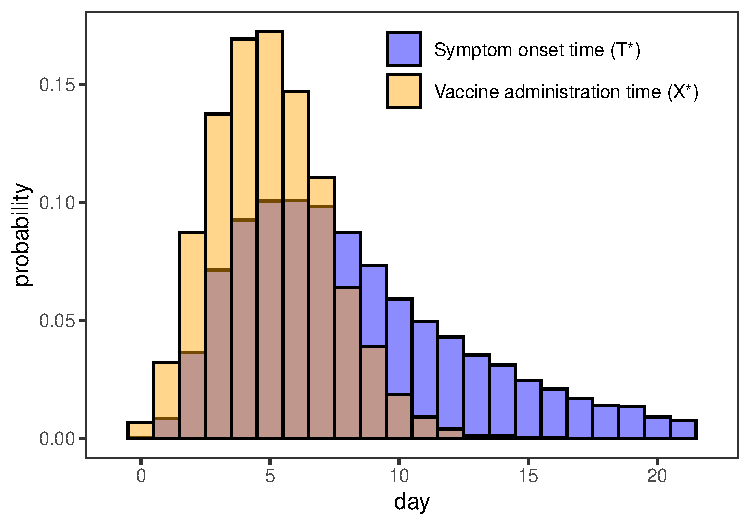
\includegraphics{../3_figures/dist.pdf}
    \caption{Distribution of simulated vaccination times ($X^*$) among vacccinated and symptom onset times ($T^*$) among the cases over the 21 days of follow up showing the degree of overlap.}
    \label{fig:sim_overlap}
\end{figure}

In each simulation, we estimate vaccine efficacy using four different strategies:
\begin{enumerate}
    \item \textit{naive} - a simple comparison of the ``ever vaccinated'' and ``never vaccinated'' using the relative risk regression model $\Pr[Y \mid X] = \operatorname{exp}\{\beta_0 + \beta_1 I(X < 21)\}$ and vaccine efficacy is estimated as $\widehat{VE} = 1 - \exp(\widehat{\beta_1})$.
    \item \textit{cox} - use a time-varying cox model $\lambda(t|X) = \lambda_0(t) \exp\{\beta_1 I(X \geq t)\}$ in which follow up time is split for vaccinated participants at the time of vaccination. Prior to this their person time is classified as unvaccinated and efficacy is estimated as $\widehat{VE} = 1 - \exp(\widehat{\beta_1})$.
    \item \textit{target trial} - emulate a sequence of nested daily trials by taking those who are symptom free and unvaccinated prior to start and compare those are vaccinated on that day to those who are not. In each trial, we censor the unvaccinated when they become vaccinated and use inverse-probability of censoring weights to account for informative censoring. These nested trials are pooled and vaccine effectiveness is estimated using pooled logistic regression $\Pr[D_{k+1} \mid A_k, \overline{D}_{k} = 0] = \operatorname{expit}(\sum_{j=0}^k \beta_{0, j} + \beta_1 A_k)$ and standard errors are estimated using cluster-robust variance estimator.
\end{enumerate}

We draw datasets of size 3000 and repeat the process 5,000 times to estimate the bias and mean squared error of each estimation strategy. In Figure \ref{fig:sim_results} we compare estimates to the truth across the three scenarios. Under the null, the naive approach is upwardly biased due to immortal time bias (i.e. by definition vaccinated have to survive long enough to be vaccinated while unvaccinated are at risk at all time points), while both the time-dependent Cox and target trial approaches yield valid estimates. The bias of the naive approach continues in scenario 2 where $VE = 40\%$, although the degree of bias is somewhat reduced by the fact that those vaccinated after developing symptoms are included with vaccinated. In scenario 3, where vaccine efficacy varies with postexposure timing, the naive and time-dependent Cox models produce biased estimates, while the target trial approach yields unbiased estimates of vaccine effectiveness. The mean squared error of the target trial estimates is comparable to that of the time-dependent Cox model, but lower than that of the naive approach. These results suggest that the target trial approach can provide valid estimates of vaccine effectiveness even when there is overlap between vaccination timing and the timing of symptom onset, and vaccine efficacy varies with postexposure timing.

\begin{figure}[t]
    \centering
    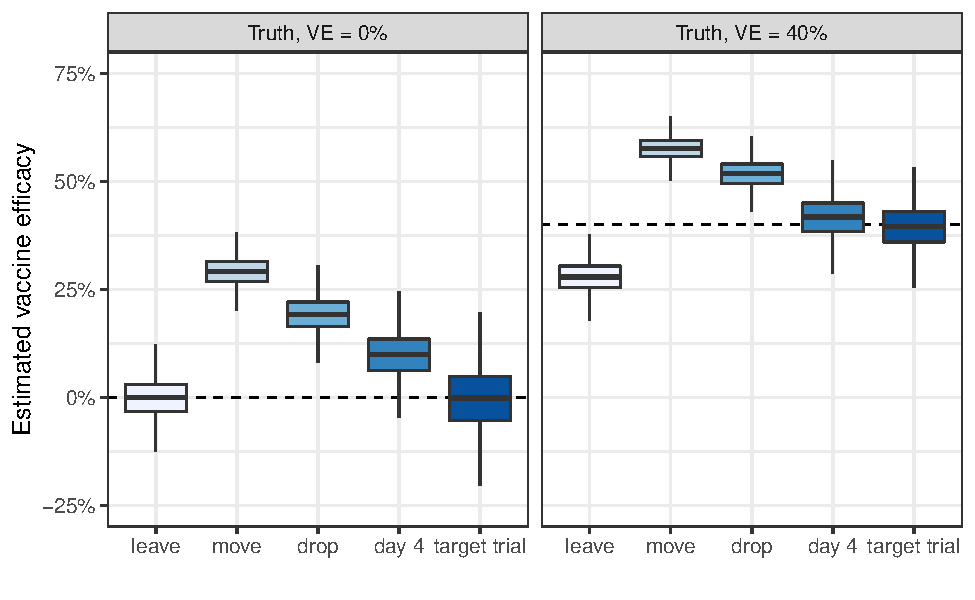
\includegraphics{../3_figures/sim.pdf}
    \caption{.\label{fig:sim_results}}
\end{figure}

In addition to comparing the estimation strategies, we also evaluate the impact of the degree of overlap between vaccination and symptom onset on the performance of the different approaches. Specifically, we vary the mean of the log-normal distribution used to generate the symptom onset times, with larger means corresponding to later sypmtom onset and thus less overlap. In the appendix, we show that the bias of the naive approach increases with the degree of overlap while both the target trial and time-dependent Cox approaches remain unbiased. This suggests that the target trial approach may be particularly useful in settings with high overlap between vaccination and symptom onset.

% Here, we consider the emulation of a target trial designed to estimate the effect of postexposure vaccine (PEV) therapy on the $\Delta$-day risk of clinical disease. The time index $t$ will denote days since exposure. We have available observational data $O=\left(L_0, A_0, D_1, \ldots, L_K, A_K, D_{K+1}\right)$ on participants, where $L_0$ includes all data prior to time zero (i.e. pre-exposure). We define the following $\{0,1\}$ dichotomous variables:
% $$A_t: A_t=1 \text{ if received vaccine at }t,$$
% $$D_t: D_t=1 \text{ if clinical disease is diagnosed at or before }t$$
% The trial outcome $Y_{t, \Delta}$ is the development of clinical disease within $\Delta$ days from randomization i.e. $Y_{t, \Delta}=D_{t+\Delta}$. Each participant is randomized with probability $1 / 2$ to the arm $G=g^*$ where $g^*$ is the regime receive PEV at time $t$ post exposure or to $G=g^{\prime}$, where $g^{\prime}$ is the regime never receive PEV beginning at $t$.

% We take as our target of interest the $t$-specific multiplicative counterfactual contrast
% $$
% \beta_{t, \Delta, S}^{\left(g^*, g^{\prime}\right)}=\log \frac{E\left\{Y_{t, \Delta}\left(g^*\right) \mid S_t\right\}}{E\left\{Y_{t, \Delta}\left(g^{\prime}\right) \mid S_t\right\}} .
% $$
% Here $Y(g)$ is the potential outcome under regime $g$ and $S_t \subset H_t=\left(\bar{L}_t, \bar{A}_{t-1}\right)$ is a vector of covariates chosen by an investigator wishing to determine whether these covariates modify the effect of treatment on this scale. If we actually had data from a true target trial we could identify $\beta_{t, \Delta, S}^{\left(g^*, g^{\prime}\right)}$ by
% $$
% \log \frac{E\left\{Y_{t, \Delta} \mid S_t, G=g^*\right\}}{E\left\{Y_{t, \Delta} \mid S_t, G=g^{\prime}\right\}} .
% $$

% Trialists are confronted with the following problem. In an ideal trial participants would be enrolled, randomized, and vaccinated immediately upon exposure. In practice, this is logistically infeasible therefore participants often receive the vaccine with some delay.

% However, by definition, the regime assignment indicator variable $G$ does not exist in the observational data $O$ since there was no randomization at $t=4$, or indeed, at any other time! Hence there is no particular reason to privilege $t=4$ rather than any other value of $t$. That is, for the particular choice of regimes $g^*$ and $g^{\prime}$ above, the observational data can be used to emulate a series of $K-\Delta+2$ target trials with enrollment at $t=0, \ldots, K-\Delta+1$ and estimands $\beta_{t, \Delta, S}^{\left(g^*, g^{\prime}\right)}$. Each eligible participant in the observational data is enrolled in each of $T-\Delta+2$ target trials.

%\section{Results} \label{sec:results}


\section{Discussion} \label{sec:discussion}
Accurate assessments of postexposure efficacy of vaccines against the onset of disease could be useful for curbing worst sequelae of many pathogens, but trials are often infeasible due to logistical, regulatory, or financial constraints. Here, we specified target trials for postexposure vaccination and describe how to emulate them using observational data. Using the example of mpox vaccines, we discussed some of the unique challenges of emulating postexposure vaccination trials, including the central role played by the distribution of vaccination times and the incubation period. Throughout we emphasize the clarifying role of the target trial framework and conclude with simulations showing how emulating the trial can help avoid several common biases in observational analyses. 

Previous studies have emulated trials of pre-exposure vaccines, particularly during the COVID-19 pandemic. These studies filled gaps in the literature by emulating trials which were not feasible to implement in practice such as head-to-head comparisons of vaccines \cite{dickerman_comparative_2022}, effectiveness against new variants \cite{cohen-stavi_bnt162b2_2022}, effectiveness of boosters \cite{barda_effectiveness_2021,magen_fourth_2022}, and effectiveness in important subgroups such as children \cite{cohen-stavi_bnt162b2_2022} and the immunocompromised. Observational emulations of post-exposure vaccines could perform a similar function.

We have mostly considered postexposure trials where the goal of vaccination is to prevent the onset of clinical disease. However, other goals such as reducing severity or transmission are also possible. To emulate trials in which the goal is to reduce severity, one could simply replace onset with an alternative outcome such as hospitalization or death in the trials outlined above. 

As shown in our simuation, some issues related to immortal time bias could be resolved by alternative estimation strategies, such as using a time-dependent Cox model. However, emulating a specific target trial helps clarify other ambiguities, provides a standard against which we can benchmark, and helps us understand when adjustment for time-varying confounding is necessary.


% \begin{itemize}
%     \item target trial framework has been used in studies of pre-exposure vaccine efficacy.
%     \item We could also consider emulating trials to compare postexposure vaccines, to estimate effectiveness against different strains or variants of the pathogen, or in different subgroups. Fill the gap.
%     \item 
%     \item could talk about adaptions necessary for effectiveness against transmission and/or severe disease.
%     \item limitations
%     \begin{itemize}
%         \item doesn't solve the issue of confounding, thoughtful adjustment, negative controls can help.
%         \item measurement of primary exposure may be difficult or there may be repeated exposure. Leads to measurement error.
%         \item in practice may be difficult to 
%         \item lack of blinding may be important in this case (think about how monitoring of those not exposed to vaccine is done).
%     \end{itemize}
    
%     \item negative control/proximal inference:
%     \begin{itemize}
%         \item If something is known about how long it takes vaccine to provoke helpful immune response then it could be that effectiveness in first X days postvaccination could be negative control.
%         \item Effects on other outcomes associated with health seeking but not vaccination.
%     \end{itemize}
% \end{itemize}
% Clarifying estimands:

% \begin{itemize}
%     \item What is the \textit{optimal} day post-exposure to receive a vaccine?
%     $$ 1 - \frac{\Pr[Y^{x = 1} = 1]}{\Pr[Y^{x \geq \Delta} = 1]} \text{ vs. } 1 - \frac{\Pr[Y^{x = 4} = 1]}{\Pr[Y^{x \geq \Delta} = 1]}$$ 
%     \item Given that I haven't developed clinical disease yet, how effective would receiving a vaccine today be?
%     $$1 - \frac{\Pr[Y^{x = 2} = 1 \mid X \geq 2]}{\Pr[Y^{x \geq \Delta} = 1 \mid X \geq 2]} \text{ vs. } 1 - \frac{\Pr[Y^{x = 5} = 1 \mid X \geq 5]}{\Pr[Y^{x \geq \Delta} = 1 \mid X \geq 5]}$$ 
%     \item What is the (average) effectiveness of receiving a vaccine \textit{within} the first $\delta$ days post-exposure?
%     $$ 1 - \frac{\Pr[Y^{x \leq 4} = 1]}{\Pr[Y^{x \geq \Delta} = 1]}\text{ vs. } 1 - \frac{\Pr[Y^{x \leq 7} = 1]}{\Pr[Y^{x \geq \Delta} = 1]}$$
% \end{itemize}
% First is probably not interesting here as, biologically, one would assume earlier vaccination is probably uniformly better. The second and third seem relevant questions though.

% $$VE(x=1) = 1 - \frac{\Pr[Y^{x = 1} = 1]}{\Pr[Y^{x \geq \Delta} = 1]} $$ 
% $$VE(x=2) = 1 - \frac{\Pr[Y^{x = 2} = 1]}{\Pr[Y^{x \geq \Delta} = 1]} $$ 

% $$VE(z) = 1 - \frac{\Pr[Y^{z = 1} = 1]}{\Pr[Y^{z = 0} = 1]} $$

% $$\Pr[Y^{\overline{a} = 1} = 1] \text{ vs. } \Pr[Y^{\overline{a} = 0} = 1]$$


% \begin{figure}[p]
%     \centering
%     \begin{tikzpicture}[> = stealth, shorten > = 1pt, auto, node distance = 2.5cm, inner sep = 0pt,minimum size = 0.5pt, semithick]
%     \tikzstyle{every state}=[
%       draw = white,
%       fill = white
%     ]
%     \node[state] (l0) {$L$};
%     \node[state] (a0) [right of=l0] {$A$};
%     \node[state] (y1) [right of=a0] {$Y$};
%     \node[state] (p0) [below of=l0] {$P$};
%     \node[state] (u0) [above of=l0] {$U$};

%     \path[->] (l0) edge node {} (a0);
%     \path[->] (l0) edge [out=20, in=160, looseness=1.5] node {} (y1);

%     \path[->] (a0) edge node {} (y1);
    
%     \path[->] (p0) edge node {} (y1);

%     \path[->] (u0) edge node {} (y1);
%     \path[->] (u0) edge node {} (l0);
%     \end{tikzpicture}
%     \caption{Example .}
%     \label{fig:dag1}
% \end{figure}

% \begin{table}[p]
%     \centering

%     \begin{threeparttable}
%         \begin{tabular}{lrrr}
%         \toprule
%         Estimator & Unweighted MSE & Weighted MSE & True MSE\\
%         \midrule
%         OLS, misspecified & 16.8 & 17.5 & 17.5\\
%         OLS, correct & 2.9 & 3.6 & 3.6\\
%         WLS, misspecified & 19.5 & 15.0 & 15.0\\
%         WLS, correct & 5.5 & 1.0 & 1.0\\
%         \bottomrule
%         \end{tabular}
%         \begin{tablenotes}
%         \item \noindent Correctly specified and incorrectly specified refers to the specification of the posited prediction model. OLS = model estimation using ordinary least squares regression (unweighted); WLS = model estimation using weighted least squares regression with weights equal to the inverse probability of being untreated. Results were averaged over 10,000 simulations. The true counterfactual MSE was obtained using numerical methods. 
%         \end{tablenotes}
%         \end{threeparttable}
    
% \end{table}

\clearpage

\newpage

% \begin{align*}
%     \frac{\Pr[I_1^{v_0, 0} = 1 \mid V_0 = v_0]}{\Pr[I_1^{0, 0} = 1 \mid V_0 = v_0]} &= \exp(\psi_{1,1} v_0) \\
%     \frac{\Pr[I_1^{v_0, v_1} = 1 \mid V_0 = v_0, I_0 = i_0, V_1 = v_1]}{\Pr[I_1^{v_0, 0} = 1 \mid V_0 = v_0, I_0 = i_0, V_1 = v_1]} &= \exp(\psi_{2,1} v_1 + \psi_{2,2} v_1 i_0 + \psi_{2,3} v_1 v_0 + \psi_{2,4} v_1 i_0 v_0) 
% \end{align*}

% \begin{align*}
%     \frac{\Pr[I_1^{v_0, 0, 0} = 1 \mid V_0 = v_0]}{\Pr[I_1^{0, 0, 0} = 1 \mid V_0 = v_0]} &= \exp(\psi_{1,1} v_0) \\
%     \frac{\Pr[I_1^{v_0, i_0, 0} = 1 \mid V_0 = v_0, I_0 = i_0]}{\Pr[I_1^{v_0, 0, 0} = 1 \mid V_0 = v_0, I_0 = i_0]} &= \exp(\psi_{2,1} i_0 + \psi_{2,2}i_0 v_0) \\
%     \frac{\Pr[I_1^{v_0, i_0, v_1} = 1 \mid V_0 = v_0, I_0 = i_0, V_1 = v_1]}{\Pr[I_1^{v_0, i_0, 0} = 1 \mid V_0 = v_0, I_0 = i_0, V_1 = v_1]} &= \exp(\psi_{3,1} v_1 + \psi_{3,2} v_1 i_0 + \psi_{3,3} v_1 v_0 + \psi_{3,4} v_1 i_0 v_0) 
% \end{align*}


\printbibliography

% \subfile{supplement.tex}

\onehalfspacing

\end{document}